\subsection{Gaussian Processes}

Gaussian processes (GPs) are a machine learning framework that considers all possible functions that could approximate a dataset, assigning a probability to each function~\cite{rasmussen2006gaussian}. The key assumption underlying GPs is that similar input points should have similar outputs, allowing the model to provide certainty estimates for specific predictions while accounting for the fact that distant points may behave differently.

GPs are defined by two functions:

\begin{enumerate}[noitemsep]
    \item \textbf{The mean function $\mu(\mathbf{x})$}, which represents prior beliefs about the underlying function
    \item \textbf{The covariance kernel $k(\mathbf{x}, \mathbf{x}')$}, which represents the correlation between two points
\end{enumerate}

GPs make predictions by providing both a posterior mean representing the predicted value and a variance represneting the uncertainty in that prediction.

\subsubsection{Kernels}
The kernel function is used to define the covariance matrix by encoding the correlation between two points. 
The choice of kernel function is crucial in GP modeling as it encodes assumptions about the smoothness, periodicity, and other properties of the underlying function. \cite{martens2016gpis}

\paragraph{Squared Exponential (RBF) Kernel}
The squared exponential kernel is defined as:
\begin{equation}
k_{SE}(\mathbf{x}, \mathbf{x}') = \sigma^2 \exp\left(-\frac{1}{2\ell^2} |\mathbf{x} - \mathbf{x}'|^2\right)
\end{equation}
where $\sigma^2$ is the signal variance and $\ell$ is the length scale parameter.

This kernel is particularly valuable for GPIS because it produces infinitely differentiable, smooth surfaces. The length scale parameter $\ell$ provides intuitive control over the surface characteristics: smaller values create surfaces that vary rapidly between points, while larger values enforce smoother transitions. This interpretability and flexibility make it well-suited for representing natural objects with continuous, smooth boundaries.

The two kernel equations are take from \textcite{martens2016gpis}.

\paragraph{Thin Plate Spline Kernel}
The thin plate spline kernel for the 3D case is given by:
\begin{equation}
k_{TP}(\mathbf{x}, \mathbf{x}') = 2d^3 - 3Rd^2 + R^3
\end{equation}
where $d = |\mathbf{x} - \mathbf{x}'|^2$ and $R$ is a hyperparameter defining the support radius.

This kernel is motivated by minimizing bending energy, analogous to the deformation of a physical thin plate. For GPIS, this property is advantageous as it naturally produces surfaces with minimal curvature, leading to smooth interpolations between sparse data points. However, unlike the squared exponential kernel, its effectiveness is limited to a finite domain characterized by $R$, and it offers less flexibility in tuning surface properties.

\subsubsection{Conditioning}
Conditioning a Gaussian process involves incorporating observed data to refine predictions. The conditioning and sampling equations are derived in both \textcite{martens2016gpis} and \textcite{seyb24from}; we adopt the notation from \textcite{seyb24from} as it is more explicit. Given measurements $\mathbf{m}$ at locations $\mathbf{C}$, the conditioned posterior GP is derived as:
\begin{equation}
f \sim \text{GP}\left(\mu|_{\zeta_m}(\mathbf{x}), k|_{\zeta_m}(\mathbf{x}, \mathbf{y})\right)
\end{equation}
where:
\begin{align}
\mu|_{\zeta_m}(\mathbf{x}) &= \mu(\mathbf{x}) + k(\mathbf{x}, \mathbf{C})k(\mathbf{C}, \mathbf{C})^{-1}(\mathbf{m} - \mu(\mathbf{C})) \\
k|_{\zeta_m}(\mathbf{x}, \mathbf{y}) &= k(\mathbf{x}, \mathbf{y}) - k(\mathbf{x}, \mathbf{C})k(\mathbf{C}, \mathbf{C})^{-1}k(\mathbf{C}, \mathbf{y})
\end{align}

\subsubsection{Sampling}

Sampling from a Gaussian process can be performed directly using:

\begin{equation}
f(\mathbf{X}) = \mu(\mathbf{X}) + k(\mathbf{X}, \mathbf{X})^{1/2}\boldsymbol{\eta}
\end{equation}

where
\begin{itemize}[noitemsep]
    \item $\boldsymbol{\eta} \sim \mathcal{N}(0, 1)$
    \item $\mathbf{A}^{1/2}$ is the matrix square root such that $\mathbf{A} = \mathbf{A}^{1/2}\mathbf{A}^{1/2}$
\end{itemize}

\subsection{Implicit Surfaces}

An \textbf{implicit surface} is defined by a function $f(X)$ where the surface exists at all points where $f = 0$. Points where $f > 0$ are conventionally inside an object and $f < 0$ are outside (though this convention can be reversed). This representation is popular because implicit surfaces are smooth, can be appropriately constrained by known geometry, and require no special treatment for topology changes. \cite{williams2007gaussian,martens2016gpis}

\subsubsection{Gaussian Process Implicit Surfaces (GPIS)}

Gaussian Process Implicit Surfaces (GPIS) were introduced by \textcite{williams2007gaussian} as a probabilistic approach to surface reconstruction~\cite{martens2016gpis}. The Gaussian process mean will decribe a manifold representing the assets.

The training data for a GPIS consists of:

\begin{itemize}[noitemsep]
    \item A set of points on the surface (where $f = 0$)
    \item A set of known points inside the surface (where $f > 0$)
    \item A set of known points outside the surface (where $f < 0$)
\end{itemize}

If we have points with associated normal vectors, we can automatically generate inside and outside points by moving a small distance along and against the normal direction.

The Gaussian process learns a function that passes smoothly through all observed points by interpolating between them. The mean of the GP represents the most likely implicit surface function, while the variance provides uncertainty estimates. The implicit surface corresponds to all points where $f(X) = 0$.


\textbf{Thin Plate Covariance Kernel}: \textcite{williams2007gaussian} derived a covariance kernel equivalent to the thin plate spline regularizer. For 3D surfaces, the thin plate kernel is:

\begin{equation}
k_{tp}(\mathbf{x}, \mathbf{x}') = 2d^3 - 3Rd^2 + R^3
\end{equation}

where $d = ||\mathbf{x} - \mathbf{x}'||$ is the distance between points and $R$ is a hyperparameter. This kernel is positive semi-definite and symmetric, ensuring that the resulting covariance matrix is valid for Gaussian process inference.

The thin plate kernel encourages smoothness by penalizing the bending energy of the surface, measured by the integral of squared second-order derivatives. This property makes it particularly well-suited for surface reconstruction tasks. \cite{martens2016gpis}

\subsubsection{Asset Representation Using Gaussian Processes}

GPIS are particularly interesting for representing shapes scanned from LiDAR data or RGB-D cameras. From a point cloud, you can condition the Gaussian process by setting the points of the point cloud as observations (with $f = 0$). This creates a manifold that can be rendered using ray marching algorithms by root finding to determine the intersection with the manifold defined by $f(X) = 0$.

For mesh-based assets, we can condition the GP by:

\begin{enumerate}[noitemsep]
    \item Adding every vertex of the mesh as a surface observation ($f = 0$)
    \item Leveraging the vertex normals to include points outside the model ($f = -1$) and inside the model ($f = +1$) by offsetting along the normal direction
\end{enumerate}

\begin{figure}[H]
    \centering
    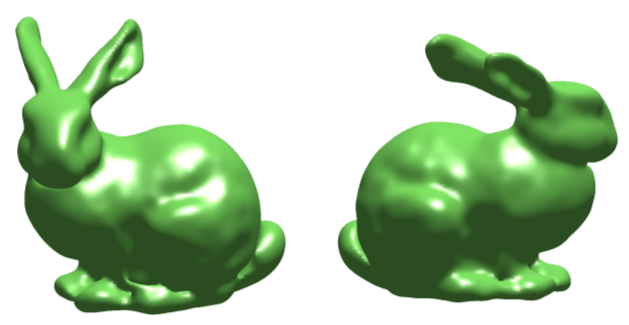
\includegraphics[width=0.5\textwidth]{img/gpis.png}
    \caption{The Stanford bunny defined by 800 surface points, one interior $+1$ point, and a sphere of 80 exterior $-1$ points generated by the marching cubes algorithm. Image from \textcite{williams2007gaussian}.}
    \label{fig:gpis_surfaces}
\end{figure}

For point clouds from LiDAR scans, the normals and the inside/outside points must be deduced from the local geometry. This can be done by estimating surface normals by using the gradient of the Gaussian process. \cite{martens2016gpis}

The resulting conditioned GP defines an implicit surface that smoothly interpolates the observed data while providing uncertainty estimates away from the observations. This probabilistic representation is particularly valuable for handling noisy sensor data and sparse observations.

\subsubsection{Derivatives of Gaussian Processes and Surface Normals}

A crucial property of Gaussian processes is that derivatives of a GP are also Gaussian processes. This property is essential for GPIS because surface normals are derived from the gradient of the implicit function.

\paragraph{Derivative Gaussian Processes}

Due to the linearity of the derivative operator, the derivative of a Gaussian process takes the form:

\begin{equation}
\text{GP}'(\mu(\mathbf{x}), k(\mathbf{x}, \mathbf{y})) = \text{GP}\left(\mu'(\mathbf{x}), k_{xy}(\mathbf{x}, \mathbf{y})\right)
\end{equation}

where:

\begin{equation}
k_{xy}(\mathbf{x}, \mathbf{y}) = \frac{\partial^2 k(\mathbf{x}, \mathbf{y})}{\partial \mathbf{x} \partial \mathbf{y}}
\end{equation}

This means we can compute the covariance between derivatives by taking the second-order cross-derivative of the original kernel function.

\paragraph{Computing Normals on GPIS}

For an implicit surface defined by $f(X) = 0$, the surface normal at any point is given by the normalized gradient:

\begin{equation}
\mathbf{n}(\mathbf{x}) = \frac{\nabla f(\mathbf{x})}{||\nabla f(\mathbf{x})||}
\end{equation}

\subsection{A Unified Theory of Light Transport with Stochastic Geometry}

Seyb et al.~\cite{seyb24from} used GPIS to define a controllable model that can represent all the elements of a scene as a continuum. This enables scene representation using a singular light transport model.

\subsubsection{Algorithm}
The path tracing algorithm for GPIS uses the ubiquitous \texttt{nextHit} function to find ray intersections. This function determines the first distance $t$ where the ray $\mathbf{x} + t\mathbf{w}$ intersects the surface, defined by $f(\mathbf{x}_t) = 0$. To find the intersection, we generate a 1D realization of the Gaussian process along the ray and locate the sign change of this 1D function. We sample the Gaussian process at $n$ points along the ray, then interpolate between these points to create a continuous 1D realization suitable for root-finding to locate the zero crossing. Once we have the intersection point, we use the previously discussed gradient technique to compute the surface normal. With both the intersection point and normal vector, we can evaluate the BSDF exactly as in a standard path tracer.
